
\documentclass[aspectratio=169]{beamer}

\usepackage{amsmath,amssymb}
\usepackage{graphicx}
\usepackage{tikz}
\usepackage{listings}
\usetikzlibrary{positioning,calc,arrows.meta,fit}

% =========================
% Colors
% =========================
\definecolor{PKUDarkPurple}{RGB}{63,63,191}
\definecolor{PKULightPurple}{RGB}{170,170,225}
\definecolor{PKUGrayBg}{RGB}{255,255,255}
\definecolor{PKUTextBlue}{RGB}{45,45,190}
\definecolor{CodeGray}{RGB}{245,245,245}
\definecolor{dkgreen}{rgb}{0,0.5,0}
\definecolor{gray}{rgb}{0.4,0.4,0.4}
\definecolor{mauve}{rgb}{0.58,0,0.82}

% =========================
% Global style
% =========================
\setbeamercolor{background canvas}{bg=PKUGrayBg}
\setbeamercolor{normal text}{fg=black,bg=PKUGrayBg}
\setbeamercolor{frametitle}{fg=PKUTextBlue,bg=PKUGrayBg}

\setbeamerfont{normal text}{size=\fontsize{15pt}{18pt}\selectfont}
\setbeamerfont{frametitle}{size=\fontsize{15pt}{19pt}\selectfont,series=\bfseries}
\setbeamerfont{itemize/enumerate body}{size=\fontsize{12pt}{15pt}\selectfont}
\setbeamerfont{itemize/enumerate subbody}{size=\fontsize{11pt}{14pt}\selectfont}
\setbeamerfont{footline}{size=\fontsize{10pt}{12pt}\selectfont}

\setbeamercolor{itemize item}{fg=PKUDarkPurple}
\setbeamertemplate{navigation symbols}{}
\setbeamertemplate{items}[ball]
\setbeamertemplate{headline}{}
\setbeamertemplate{footline}{}

% =========================
% Code style
% =========================
\lstset{
  basicstyle=\ttfamily\footnotesize,
  backgroundcolor=\color{CodeGray},
  keywordstyle=\color{blue},
  commentstyle=\color{dkgreen},
  stringstyle=\color{mauve},
  showstringspaces=false,
  breaklines=true,
  frame=single,
  columns=fullflexible
}

% =========================
% Custom headline and footline
% =========================
\newcommand{\makecustomheadline}{
\begin{tikzpicture}[remember picture,overlay]
    \fill[PKUDarkPurple]
        (current page.north west)
        rectangle
        ([xshift=.50\paperwidth,yshift=-0.35cm]current page.north west);

    \fill[PKULightPurple]
        ([xshift=.50\paperwidth]current page.north west)
        rectangle
        ([xshift=\paperwidth,yshift=-0.35cm]current page.north west);
\end{tikzpicture}
}

\newcommand{\makecustomfootline}{
\begin{tikzpicture}[remember picture,overlay]
    \fill[PKUDarkPurple]
        (current page.south west)
        rectangle
        ([xshift=.33\paperwidth,yshift=0.42cm]current page.south west);

    \fill[PKULightPurple]
        ([xshift=.33\paperwidth]current page.south west)
        rectangle
        ([xshift=.67\paperwidth,yshift=0.42cm]current page.south west);

    \fill[PKULightPurple]
        ([xshift=.67\paperwidth]current page.south west)
        rectangle
        ([xshift=\paperwidth,yshift=0.42cm]current page.south west);

    \node[anchor=center, text=white, font=\small]
        at ([xshift=.165\paperwidth,yshift=0.21cm]current page.south west)
        {\textrm{huangxun@pku.edu.cn}};

    \node[anchor=center, text=white, font=\small]
        at ([xshift=.50\paperwidth,yshift=0.21cm]current page.south west)
        {AI Enabled Control Engineering};

    \node[anchor=center, text=black, font=\small]
        at ([xshift=.83\paperwidth,yshift=0.21cm]current page.south west)
        {2026 Summer};

    \node[anchor=center, text=black, font=\small]
        at ([xshift=.965\paperwidth,yshift=0.21cm]current page.south west)
        {\insertframenumber/\inserttotalframenumber};
\end{tikzpicture}
}

\addtobeamertemplate{background}{\makecustomheadline\makecustomfootline}{}

\title{\textcolor{PKUTextBlue}{AI Enabled Control Engineering}}
\author{\textcolor{blue}{Professor Xun Huang}}
\institute{
Aeronautics and Astronautics\\
College of Engineering\\
Peking University\\[0.25cm]
huangxun@pku.edu.cn\\
https://xunger99.github.io/xunger/
}
\date{}

\setbeamertemplate{title page}{
    \vspace{1.0cm}
    \begin{center}
        {\fontsize{18}{22}\selectfont\bfseries \inserttitle\par}
        \vspace{0.3cm}
        {\fontsize{15}{18}\selectfont Lecture 9: State Observers for Control of the Rotary Inverted Pendulum\par}
          \vspace{0.3cm}
        {\fontsize{15}{18}\selectfont \insertauthor\par}
        \vspace{0.15cm}
        {\fontsize{11}{13}\selectfont TA: Zhixiang Ju \quad Haozhe Wang\par}
        \vspace{0.4cm}
        {\fontsize{8}{11}\selectfont \insertinstitute\par}
    \end{center}
}

\begin{document}

% ---------------------------------
\begin{frame}
\titlepage
\end{frame}

% ---------------------------------
\begin{frame}{Recap: from Class 8 to Class 9}
\begin{itemize}
    \item In Class 8, we used LQR and MPC to stabilize the real rotary inverted pendulum near the upright equilibrium.
    \vspace{0.25cm}
    \item The controller state was
    \[
    x_k=[\theta_k,\dot\theta_k,\alpha_k,\dot\alpha_k]^\top.
    \]
    \vspace{0.25cm}
    \item However, the hardware sensors directly measure only two angles:
    \[
    y_k=[\theta_k,\alpha_k]^\top.
    \]
    \vspace{0.25cm}
    \item The previous solution estimated angular velocities by low-pass-filtered finite differences.
\end{itemize}
\end{frame}

% ---------------------------------
\begin{frame}{Why do we need an observer?}
\begin{itemize}
    \item Direct angle difference is simple:
    \[
    \dot\theta_k\approx\frac{\theta_k-\theta_{k-1}}{T_s},\qquad
    \dot\alpha_k\approx\frac{\alpha_k-\alpha_{k-1}}{T_s}.
    \]

    \item But differentiation amplifies high-frequency sensor noise.

    \item Noisy velocity estimates may cause oscillatory PWM commands.
   
    \item An observer uses both the model and the measurements to estimate the full state.
\end{itemize}

\begin{block}{Goal of Class 9}
\small
Replace low-pass finite-difference velocities by model-based observer states, then test LQR and MPC again on the real hardware.
\end{block}
\end{frame}

% ---------------------------------
\begin{frame}{Measured output and observer state}
The local discrete model is
\[
x_{k+1}=A_dx_k+B_du_k.
\]

The measured output is
\[
y_k=Cx_k,
\qquad
C=\begin{bmatrix}
1&0&0&0\\
0&0&1&0
\end{bmatrix}.
\]

\vspace{0.2cm}
The observer estimates
\[
\hat{x}_k=
\begin{bmatrix}
\hat\theta_k & \widehat{\dot\theta}_k & \hat\alpha_k & \widehat{\dot\alpha}_k
\end{bmatrix}^\top.
\]


LQR and MPC will use \(\hat{x}_k\), not the low-pass finite-difference state.

\end{frame}

% ---------------------------------
\begin{frame}{Observer as prediction plus correction}
\begin{center}
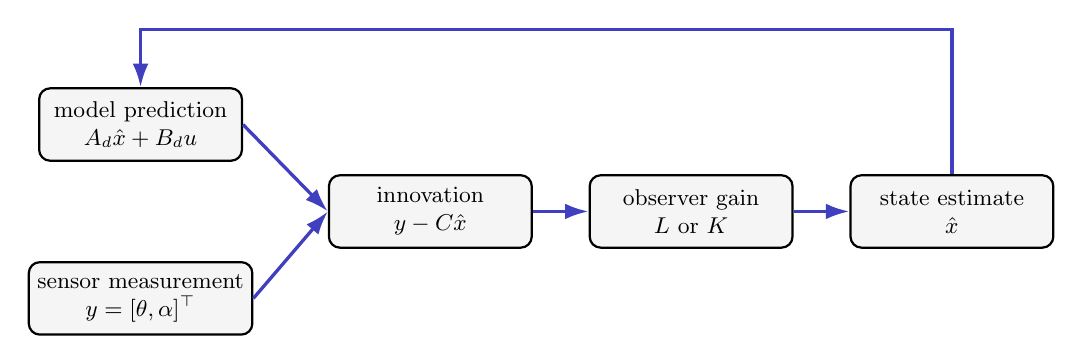
\begin{tikzpicture}[
    scale=0.92,
    transform shape,
    font=\small,
    >={Latex[length=3mm,width=2mm]},
    box/.style={draw, thick, rounded corners=4pt, align=center, minimum width=2.8cm, minimum height=1.0cm, fill=CodeGray},
    arrow/.style={->, very thick, draw=PKUDarkPurple}
]
\node[box] (model) at (0,1.2) {model prediction\\\(A_d\hat{x}+B_du\)};
\node[box] (sensor) at (0,-1.2) {sensor measurement\\\(y=[\theta,\alpha]^\top\)};
\node[box] (innovation) at (4.0,0) {innovation\\\(y-C\hat{x}\)};
\node[box] (gain) at (7.6,0) {observer gain\\\(L\) or \(K\)};
\node[box] (state) at (11.2,0) {state estimate\\\(\hat{x}\)};
\draw[arrow] (model.east) -- (innovation.west);
\draw[arrow] (sensor.east) -- (innovation.west);
\draw[arrow] (innovation.east) -- (gain.west);
\draw[arrow] (gain.east) -- (state.west);
\draw[arrow] (state.north) -- ++(0,2.0) -| (model.north);
\end{tikzpicture}
\end{center}

\vspace{0.2cm}
\begin{block}{Intuition}
\small
The model predicts how the state should evolve. The measurement corrects the prediction whenever the predicted angle disagrees with the measured angle.
\end{block}
\end{frame}

% ---------------------------------
\begin{frame}{Observability check}
For the pair \((A_d,C)\), define the observability matrix
\[
\mathcal O=
\begin{bmatrix}
C\\
CA_d\\
CA_d^2\\
CA_d^3
\end{bmatrix}.
\]

If
\[
\mathrm{rank}(\mathcal O)=4,
\]
then the four-dimensional state can be reconstructed from the angle measurements and the model dynamics.


\begin{alertblock}{For the RIP system}
\small
Although \(\dot\theta\) and \(\dot\alpha\) are not directly measured, they can be estimated because the local model with outputs \(\theta,\alpha\) is observable.
\end{alertblock}
\end{frame}

% ---------------------------------
\begin{frame}{Luenberger observer: discrete-time form}
A simple discrete Luenberger observer can be written as
\[
\hat{x}_{k}
=
(A_d-L_dC)\hat{x}_{k-1}
+B_du_{k-1}
+L_dy_k.
\]

Equivalently,
\[
\hat{x}_{k}
=
A_d\hat{x}_{k-1}+B_du_{k-1}
+L_d\left(y_k-C\hat{x}_{k-1}\right).
\]

\vspace{0.2cm}
\begin{itemize}
    \item \(A_d\hat{x}_{k-1}+B_du_{k-1}\): model prediction.
    \vspace{0.15cm}
    \item \(y_k-C\hat{x}_{k-1}\): measurement innovation.
    \vspace{0.15cm}
    \item \(L_d\): observer gain to be designed.
\end{itemize}
\end{frame}

% ---------------------------------
\begin{frame}{Luenberger observer error dynamics}
Define the estimation error
\[
e_k=x_k-\hat{x}_k.
\]

Using
\[
x_k=A_dx_{k-1}+B_du_{k-1},
\]
and the observer update, we get
\[
e_k=(A_d-L_dC)e_{k-1}.
\]

\vspace{0.25cm}
Therefore, the observer is stable if
\[
\rho(A_d-L_dC)<1,
\]
where \(\rho(\cdot)\) is the spectral radius.

\end{frame}

% ---------------------------------
\begin{frame}{How to choose Luenberger observer poles}
\begin{itemize}
    \item Observer poles should be inside the unit circle.
    \vspace{0.25cm}
    \item Faster poles give faster estimation convergence.
    \vspace{0.25cm}
    \item But poles that are too fast amplify measurement noise.
    \vspace{0.25cm}
    \item In practice, choose poles faster than the closed-loop control poles, but not extremely close to zero.
\end{itemize}

\vspace{0.2cm}
\begin{block}{Suggested starting range}
\small
Start with real or complex poles with magnitudes around \(0.5\sim0.85\), then test on LQR hardware logs.
\end{block}
\end{frame}

% ---------------------------------
\begin{frame}[fragile]{Computing \(L_d\) by pole placement}
For observer design, use the duality between controllability and observability:
\[
\mathrm{eig}(A_d-L_dC)
\quad\Longleftrightarrow\quad
\mathrm{place}(A_d^\top,C^\top,\text{poles}).
\]

\vspace{0.15cm}
In Python:
\begin{lstlisting}[basicstyle=\ttfamily\scriptsize]
from scipy.signal import place_poles

poles = [0.55+0.20j, 0.55-0.20j, 0.72, 0.82]
res = place_poles(Ad.T, C.T, poles)
Ld = res.gain_matrix.T
\end{lstlisting}

\vspace{0.15cm}
\begin{alertblock}{Student task}
\small
Try several pole sets, upload the resulting \(L_d\), and compare observer-based LQR logs.
\end{alertblock}
\end{frame}

% ---------------------------------
\begin{frame}{Luenberger observer tuning workflow}
\begin{enumerate}
    \item Choose a candidate pole set inside the unit circle.
    \vspace{0.2cm}
    \item Compute \(L_d\) using \texttt{place\_poles}.
    \vspace{0.2cm}
    \item Fill \(L_d\) into \texttt{rip\_lqr\_luenberger\_control.ino}.
    \vspace{0.2cm}
    \item Test LQR with observer state \(\hat{x}_k\).
    \vspace{0.2cm}
    \item Compare \(\alpha(t)\), PWM, and estimated velocities.
    \vspace{0.2cm}
    \item Keep the pole set that gives stable and smooth control.
\end{enumerate}
\end{frame}

% ---------------------------------
\begin{frame}{Kalman observer: stochastic model}
The discrete stochastic model is
\[
x_{k+1}=A_dx_k+B_du_k+w_k,
\]
\[
y_k=Cx_k+v_k.
\]

\vspace{0.15cm}
Here:
\begin{itemize}
    \item \(w_k\): process noise, representing model mismatch and unmodeled disturbances.
    \vspace{0.15cm}
    \item \(v_k\): measurement noise, representing sensor noise and quantization errors.
\end{itemize}

\vspace{0.15cm}
Assume
\[
E[w_kw_k^\top]=Q_n,
\qquad
E[v_kv_k^\top]=R_n.
\]
\end{frame}

% ---------------------------------
\begin{frame}{Kalman observer: prediction and correction}
Prediction:
\[
\hat{x}_{k|k-1}=A_d\hat{x}_{k-1|k-1}+B_du_{k-1}.
\]

Innovation:
\[
\nu_k=y_k-C\hat{x}_{k|k-1}.
\]

Correction:
\[
\hat{x}_{k|k}=\hat{x}_{k|k-1}+K_k\nu_k.
\]

\vspace{0.2cm}
The Kalman gain is
\[
K_k=P_{k|k-1}C^\top(CP_{k|k-1}C^\top+R_n)^{-1}.
\]

\vspace{0.1cm}
\begin{block}{Interpretation}
\small
Kalman filtering automatically balances model prediction and sensor measurement according to noise levels.
\end{block}
\end{frame}

% ---------------------------------
\begin{frame}{Steady-state Kalman observer}
For a time-invariant system, the covariance can converge to a fixed matrix \(\Pi\).

\vspace{0.15cm}
Then the Kalman gain becomes constant:
\[
K=\Pi C^\top(C\Pi C^\top+R_n)^{-1}.
\]

\vspace{0.15cm}
The embedded observer can be implemented as
\[
\hat{x}_{k|k-1}=A_d\hat{x}_{k-1}+B_du_{k-1},
\]
\[
\hat{x}_{k}=\hat{x}_{k|k-1}+K(y_k-C\hat{x}_{k|k-1}).
\]

\vspace{0.15cm}
\begin{block}{Why steady-state?}
\small
Only a fixed gain matrix is stored on STM32. No covariance matrix needs to be updated online.
\end{block}
\end{frame}

% ---------------------------------
\begin{frame}{How students tune Kalman parameters}
\begin{itemize}
    \item Choose process noise covariance \(Q_n\).
    \vspace{0.2cm}
    \item Choose measurement noise covariance \(R_n\).
    \vspace{0.2cm}
    \item Larger \(R_n\): trust sensors less, smoother but slower correction.
    \vspace{0.2cm}
    \item Larger \(Q_n\): trust model less, faster response to measurement.
    \vspace{0.2cm}
    \item Use logs to estimate sensor noise in the two measured angle channels.
\end{itemize}

\vspace{0.15cm}
\begin{block}{Practical measurement noise estimate}
\small
Hold the system still, record \(\theta\) and \(\alpha\), then compute the sample variances. These can be used as initial values for \(R_n\).
\end{block}
\end{frame}

% ---------------------------------
\begin{frame}[fragile]{Computing steady-state Kalman gain}
In Python, students can use the discrete Riccati equation:
\begin{lstlisting}[basicstyle=\ttfamily\scriptsize]
from scipy.linalg import solve_discrete_are

Pi = solve_discrete_are(Ad.T, C.T, Qn, Rn)
K  = Pi @ C.T @ np.linalg.inv(C @ Pi @ C.T + Rn)
\end{lstlisting}

\vspace{0.2cm}
Then fill \(K\) into the STM32 firmware:
\begin{lstlisting}[basicstyle=\ttfamily\scriptsize]
static const float K_KALMAN[4][2] = {
  { ... , ... },
  { ... , ... },
  { ... , ... },
  { ... , ... }
};
\end{lstlisting}

\vspace{0.1cm}
\begin{alertblock}{Student task}
\small
Try several \(Q_n,R_n\) settings and compare observer-based LQR logs first.
\end{alertblock}
\end{frame}

% ---------------------------------
\begin{frame}{Experiment strategy of Class 9}
\begin{enumerate}
    \item Start from the LQR controller.
    \vspace{0.2cm}
    \item Replace low-pass velocity difference by a Luenberger observer.
    \vspace{0.2cm}
    \item Tune \(L_d\) until LQR hardware response is stable and smooth.
    \vspace{0.2cm}
    \item Replace the observer by a steady-state Kalman observer.
    \vspace{0.2cm}
    \item Tune \(Q_n,R_n\) until Kalman-based LQR performs well.
    \vspace{0.2cm}
    \item Then apply the good observer parameters to MPC.
\end{enumerate}
\end{frame}

% ---------------------------------
\begin{frame}{Provided code packages}
\begin{center}
\begin{tabular}{c|c|c}
\hline
Package & Controller & State source \\
\hline
\texttt{class9\_lqr\_luenberger\_lab.zip} & LQR & Luenberger observer \\
\texttt{class9\_lqr\_kalman\_lab.zip} & LQR & steady-state Kalman observer \\
\texttt{class9\_mpc\_luenberger\_lab.zip} & MPC & Luenberger observer \\
\texttt{class9\_mpc\_kalman\_lab.zip} & MPC & steady-state Kalman observer \\
\hline
\end{tabular}
\end{center}

\vspace{0.25cm}
\begin{alertblock}{Important}
\small
Observer gain matrices are intentionally left as student parameters. Fill them before running the hardware experiment.
\end{alertblock}
\end{frame}

% ---------------------------------
\begin{frame}{LQR observer experiment procedure}
\begin{enumerate}
    \item Calibrate \texttt{POT\_ZERO}.
    \vspace{0.18cm}
    \item Compute LQR gain \(K\), as in Class 8.
    \vspace{0.18cm}
    \item Design observer gain \(L_d\) or Kalman gain \(K\).
    \vspace{0.18cm}
    \item Fill the gain matrix into the LQR observer firmware.
    \vspace{0.18cm}
    \item Upload firmware to STM32.
    \vspace{0.18cm}
    \item Hold the pendulum near upright and press Enter in Python.
    \vspace{0.18cm}
    \item Save CSV and compare with Class 8 low-pass-difference LQR logs.
\end{enumerate}
\end{frame}

% ---------------------------------
\begin{frame}{MPC observer experiment procedure}
\begin{enumerate}
    \item Use the observer parameters that worked well in LQR.
    \vspace{0.2cm}
    \item Fill the same observer matrix into the MPC observer firmware.
    \vspace{0.2cm}
    \item Upload MPC observer firmware to STM32.
    \vspace{0.2cm}
    \item Hold the pendulum near upright and press Enter in Python.
    \vspace{0.2cm}
    \item Compare MPC-Luenberger and MPC-Kalman logs.
\end{enumerate}

\vspace{0.2cm}

\end{frame}

% ---------------------------------
\begin{frame}{What to compare in the report}
\begin{itemize}
    \item Low-pass-difference LQR from Class 8.
   
    \item Low-pass-difference MPC from Class 8.
       
    \item Luenberger-observer LQR.

    \item Kalman-observer LQR.
 
    \item Luenberger-observer MPC.
   
    \item Kalman-observer MPC.
\end{itemize}


Recommended plots:
\[
\alpha(t),\quad \theta(t),\quad \widehat{\dot\theta}(t),\quad \widehat{\dot\alpha}(t),\quad u(t).
\]

\begin{block}{Evaluation}
\small
A good observer should give smooth velocity estimates, stable upright control, and no long-term PWM saturation.
\end{block}
\end{frame}

% ---------------------------------
\begin{frame}{Summary of Class 9}
\begin{itemize}
    \item The RIP sensors directly measure only \(\theta\) and \(\alpha\).
    \vspace{0.25cm}
    \item Direct finite difference is simple but amplifies noise.
    \vspace{0.25cm}
    \item Luenberger observers use pole placement to make estimation error converge.
    \vspace{0.25cm}
    \item Steady-state Kalman observers use noise covariance matrices to balance model prediction and sensor correction.
    \vspace{0.25cm}
    \item In the experiment, we first tune observers with LQR, then reuse good observers in MPC.
\end{itemize}

\vspace{0.15cm}
\begin{alertblock}{Take-home message}
\small
Observers are the bridge between limited hardware measurements and full-state optimal control.
\end{alertblock}
\end{frame}

\end{document}
